\documentclass[a4paper]{article}

\usepackage[english]{babel}
\usepackage[utf8]{inputenc}
\usepackage[T1]{fontenc}
\usepackage{amsmath}
\usepackage{verbatim}
\usepackage{graphicx}
\usepackage{hyperref}
\usepackage[colorinlistoftodos]{todonotes}
\usepackage{float}
\usepackage{geometry}

\title{STLDD - Software Top Level Design Document}
\author{Team 2}

\begin{document}
	\begin{titlepage}
		\newgeometry{left=2cm,top=1cm,right=2cm}
		\newcommand{\HRule}{\rule{\linewidth}{0.5mm}}
		
		\begin{minipage}{0.5\textwidth}
			\begin{flushleft} % Responsible persons, write on separate lines
				\textit{Responsible for this document:}\\
				Oscar Axelsson \\
				Daniel Olsson \\
				Jacob Mejvik
			\end{flushleft}
		\end{minipage}
		~
		\begin{minipage}{0.4\textwidth}
			\begin{flushright}
				PUSS154214 v1.0
				\today
			\end{flushright}
		\end{minipage}\\[3cm]
		
		\centering
		\textsc{\LARGE Team 2}\\[0.5cm]
		
		\HRule \\[0.4cm]
		{ \huge \bfseries Software Top Level Design Document}\\[0.4cm] % Title of your document
		\HRule \\[1.5cm]
		
		\vfill
		\begin{flushleft}
			%Authors, write on separate lines
			\textit{Authors of this document:}\\
			Jacob Mejvik \\
			Oscar Axelsson \\
			Daniel Olsson
		\end{flushleft}
		
	\end{titlepage}
	\pagenumbering{gobble}
	\setcounter{tocdepth}{2}
	
	\begin{center}
		\textit{\large Version History}
		
		\begin{tabular}{ | l | l | l | p{5cm} |}
			\hline
			\textbf{Version} 	& \textbf{Date} 	& \textbf{Responsible} 	& \textbf{Description} 		\\ \hline
			1.0				 	& 240915 			& DO, JM, OA			&  Baseline. 				\\ \hline
		\end{tabular}
	\end{center}
	
	
	\tableofcontents
	\newpage
	\pagenumbering{arabic}
	
	\section{Introduction}
	This document describes the top level design of the Lamp Controller Application. The application can connect to a light bulb and a sensor device, these devices can also be controlled and data can be received using a MVD. The application is developed as a project within the course "Software Development for Large Systems - ETSN05" at LTH.
	
	\section{Reference Documents}
	PUSS154212 - System Requirements Specification for the current project
	
	
	\section{Overview}
	The main purpose of the Lamp Controller Application is to provide an graphical interface used to control a light bulb and a sensor device from an MVD via a REST API provided by the backend. The application will provide three different views to detect and control the different devices. A UML diagram have been created to visualize the design of a system figure \ref{fig:uml}. Several sequence diagram have been created to visualize the interaction and can be viewed in figures 2-5.
	
	\subsection{Controller Application}
	\begin{itemize}
		\item{\textbf{BaseActivity:}} 
		The BaseActivity for the application that will connect the Activities with the NetworkManager. Is an abstract class that both DeviceActivity and MyDeviceActivity inherits from.
		\item{\textbf{MyDeviceActivity:}} 
		Is the start screen of the application. Will contain a ListView and has methods for detecting devices and control a device that was selected from the ListView.
		\item{\textbf{DeviceListAdapter:}} 
		Adapter that handles the list in MyDevicesActivity, the ListView can display any data provided that it is wrapped in a ListAdapter.\\ 
        - void addDevices(List<Device>) will add a list of devices to the adapter to display it in the activity.
		\item{\textbf{Device:}} 
		Is an abstract class that contains information about the two devices we are handling. \\
        - String getMacAddress() returns the String MacAddress value of a Device.\\
        - String getId() returns the String id number of a Device.\\
        - String getName() Is an abstract method that is declared without an implementation in this class.
		\item{\textbf{SensorDevice:}} 
		Class containing the SensorDevice information.\\
        - String getName() returns the String Name of a Device.
		\item{\textbf{LightBulb:}}
		Class containing the LightBulb information.\\
        - String getName() returns the String Name of a Device.
		\item{\textbf{DeviceActivity:}} 
		Is an abstract class that holds the protected parameters deviceName, id and macAddress.\\
		- void toggle(boolean) is a method that controls the on/off switch of the Devices set by the boolean value.
		\item{\textbf{SensorDeviceActivity:}} 
		Is the controller in the interaction with the user in the SensorDeviceAcitvity. Handles the TextView fields and the buttons that will retrieve and present the information regarding the sensors from NetworkManager.
		\item{\textbf{LightBulbActivity:}} 
		Is the controller in the interaction with the user in the LightBulb View. Handles the EditText fields and the buttons that will retrieve and send information from/to the NetworkManager.
		
		\item{\textbf{NetworkManager:}} 
		Handles all the communication with the API to access the backend. There are different methods for both receiving and setting data values.\\
        - void toggle(Device, boolean, Callback<Response>) sets the on/off switch of the Device to the boolean value. Returns the response using a Callback.\\
        - void getToggleState(Device, Callback<Response>) returns the state of the toggle received from the API using a Callback. Device attribute to know to which host the connection should be made and which device the toggle conserns.\\
        - void detectDevices(List<Device>, Callback<DeviceResponse>) will return a List of Devices that will be displayed in the MyDeviceActivity using the adapter.\\
        - void getTemperature(Device, Callback<TemperatureResponse>) returns the Temperature received from the API using a Callback. Device attribute to know to which host the connection should be made.\\
        - void getPressure(Device, Callback<PressureResponse>) returns the Pressure received from the API using a Callback. Device attribute to know to which host the connection should be made.\\
        - void getHumidity(Device, Callback<HumidityResponse>) 
        returns the Humidity received from the API using a Callback. Device attribute to know to which host the connection should be made.\\
        - void getMagnetic(Device, Callback<MagneticResponse>) returns the Magnetic received from the API using a Callback. Device attribute to know to which host the connection should be made.\\
        - void getGyroscopic(Device, Callback<GyroscopicResponse>) returns the Gyroscopic received from the API using a Callback. Device attribute to know to which host the connection should be made.\\
        - void getAccelerometer(Device, Callback<AccelerometerResponse>) returns the Accelerometer received from the API using a Callback. Device attribute to know to which host the connection should be made.\\
        - void getAllSensorValues(Device, Callback<AllSensorValuesResponse>) returns all the sensor values that could be retrieved from the API using a Callback. Device attribute to know to which host the connection should be made.\\
        - void getColor(Device, Callback<GetColorResponse>) returns the Color received from the API using a Callback. Device attribute to know to which host the connection should be made.\\
        - void setColor(Device, Color color,  Callback<ColorResponse>) sets the color of the light bulb. Device to receive the correct host, Color to set the color and a Callback that will return from the API network.
		\item{\textbf{SensorValues:}} 
		A class the handles the information of the different sensors.\\
        - Temperature getTemperature() returns the class Temperature that has information regarding the temperature.\\
        - Pressure getPressure() returns the class Pressure that has information regarding the pressure data.\\
        - Humidity getHumidity() returns the class Humidity that has information regarding the humidity data.\\
        - Magnetic getMagnetic() returns the class Magnetic that has information regarding the magnetic data.\\
        - Gyroscopic getGyroscopic() returns the class Gyroscopic that have information regarding the gyroscopic data.\\
         - Accelerometer getAccelerometer() returns the class Accelerometer that has information regarding the accelerometer data.
	\item{\textbf{Temperature:}} 
    Handles the information regarding the temperature data.
    \item{\textbf{Pressure:}} 
    Handles the information regarding the pressure data.
    \item{\textbf{Humidity:}} 
    Handles the information regarding the humidity data.
    \item{\textbf{Magnetic:}} 
    Handles the information regarding the magnetic data.
    \item{\textbf{Gyroscopic:}} 
    Handles the information regarding the gyroscopic data.
    \item{\textbf{Accelerometer:}} 
    Handles the information regarding the accelerometer data.
	\end{itemize}

	\subsection{Packages}
	\begin{itemize}
		\item {\textbf{Network}} \\
        Handles the network communication and contains the class NetworkManager.
		\item {\textbf{Activity}}\\
        Handles the Activities for the different views. Contains the classes BaseActivity, DeviceActivity, MyDeviceActivity, SensorDeviceActivity and LighBulbActivity.
		\item {\textbf{Adapter}}\\
        The Adapter to the ListView used in MyDeviceActivity contains the class DeviceListAdapter.
		\item {\textbf{Model}}\\
        Handels the information about the different devices contains the classes Device, SensorDevice and LightBulb, SensorValues, Temperature, Pressure, Humidity, Magnetic, Gyroscopic and Accelerometer.
	\end{itemize}
\subsection{UML diagram}
	\begin{figure}[H]
    \centering
    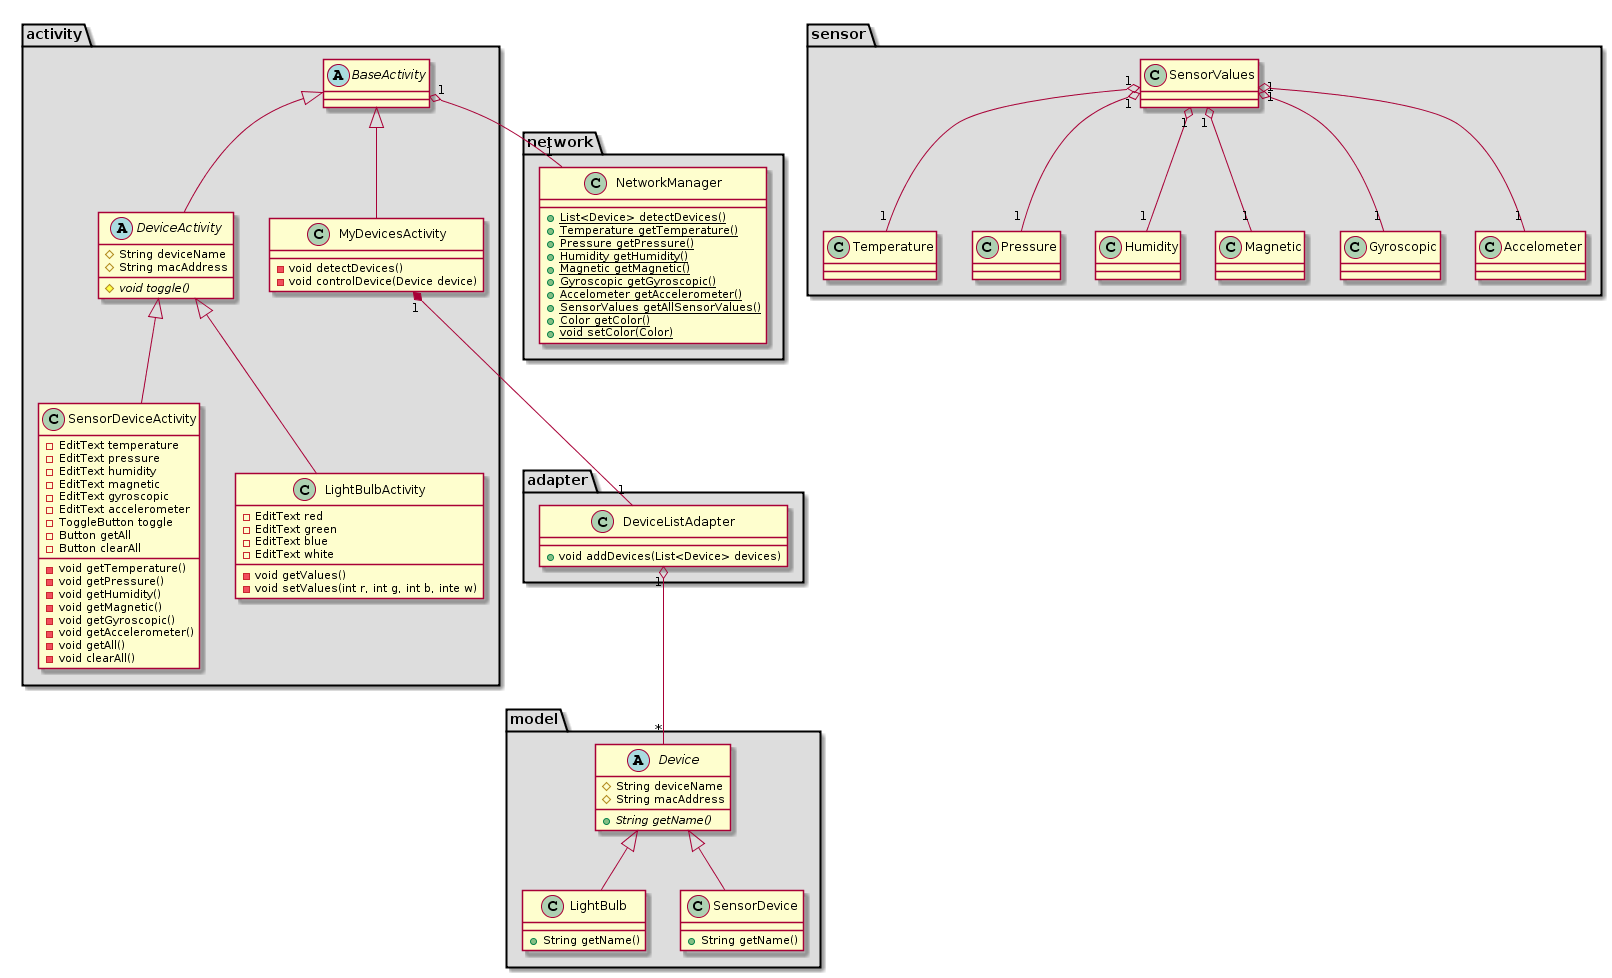
\includegraphics[width=0.8\textwidth]{class_diagram.png}
    \caption{The design of the system.}
    \label{fig:uml}
\end{figure}

	
	\subsection{Sequence diagrams}
	The red arrows show internal calls within the application. The blue arrows shows communication outside the app which is with the MVD.
	
	\begin{figure}[H]
    \centering
    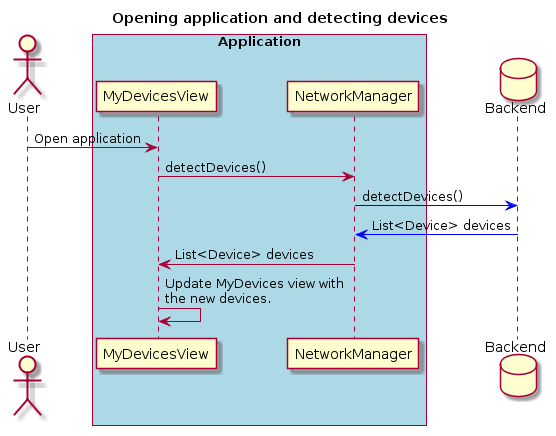
\includegraphics[width=0.6\textwidth]{seq.png} 
    \caption{Opening application and detecting devices.}
    \label{fig:seq}
\end{figure}

\begin{figure}[H]
    \centering
    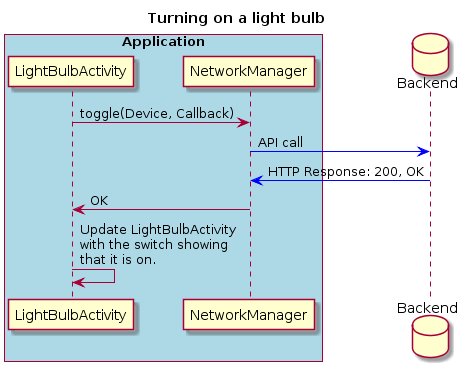
\includegraphics[width=0.6\textwidth]{seq1.png}
    \caption{Turn on the light bulb with the user located in the LightBulbActivity.}
    \label{fig:seq1}
\end{figure}

\begin{figure}[H]
    \centering
    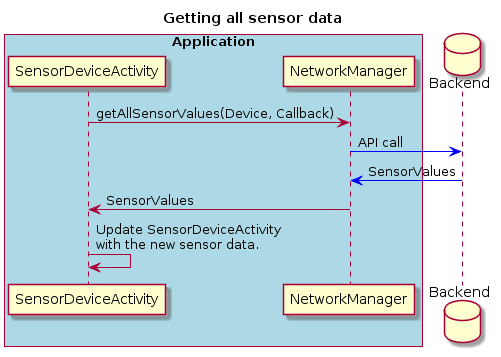
\includegraphics[width=0.6\textwidth]{seq2.png}
    \caption{Get all sensor data with the user located in the SensorDeviceActivity.}
    \label{fig:seq2}
\end{figure}

\begin{figure}[H]
    \centering
    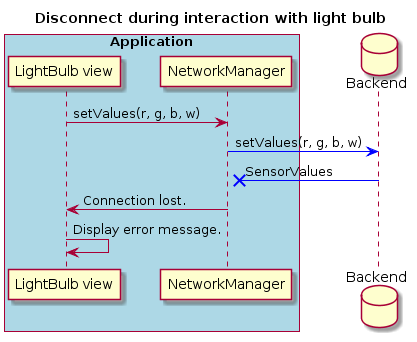
\includegraphics[width=0.6\textwidth]{seq3.png}
    \caption{Set color of light bulb with the user located in the LightBulb view and the backend is unresponsive.}
    \label{fig:seq3}
\end{figure}
	
\end{document}